% === DEN Brand Colors ===
\usepackage{xcolor}
\definecolor{denbrown}{HTML}{6A4A3C}
\definecolor{dendark}{HTML}{2B2B2B}
\definecolor{dengray}{HTML}{F2F2F2}

% === Required Packages ===
\usepackage{tikz}
\usepackage{graphicx}
\usepackage{calc}

% === Beamer Theme Settings ===
\usetheme{default}
\usecolortheme{default}

% Remove navigation symbols
\setbeamertemplate{navigation symbols}{}

% === Font Settings ===
\usefonttheme{professionalfonts}
\setbeamerfont{title}{size=\LARGE, series=\bfseries}
\setbeamerfont{frametitle}{size=\large, series=\bfseries}
\setbeamerfont{framesubtitle}{size=\normalsize}

% === Color Settings ===
\setbeamercolor{normal text}{fg=dendark}
\setbeamercolor{frametitle}{fg=dendark}
\setbeamercolor{title}{fg=white}
\setbeamercolor{author}{fg=white}
\setbeamercolor{date}{fg=white}
\setbeamercolor{item}{fg=denbrown}
\setbeamercolor{itemize item}{fg=denbrown}
\setbeamercolor{enumerate item}{fg=denbrown}

% === Adaptive Title Sizing ===
\usepackage{ifthen}
\newlength{\titlewidth}
\newlength{\titlemaxwidth}

% === Title Page Template with Adaptive Sizing ===
\setbeamertemplate{title page}{
  \begin{tikzpicture}[remember picture, overlay]
    \node[anchor=center] at (current page.center) {
      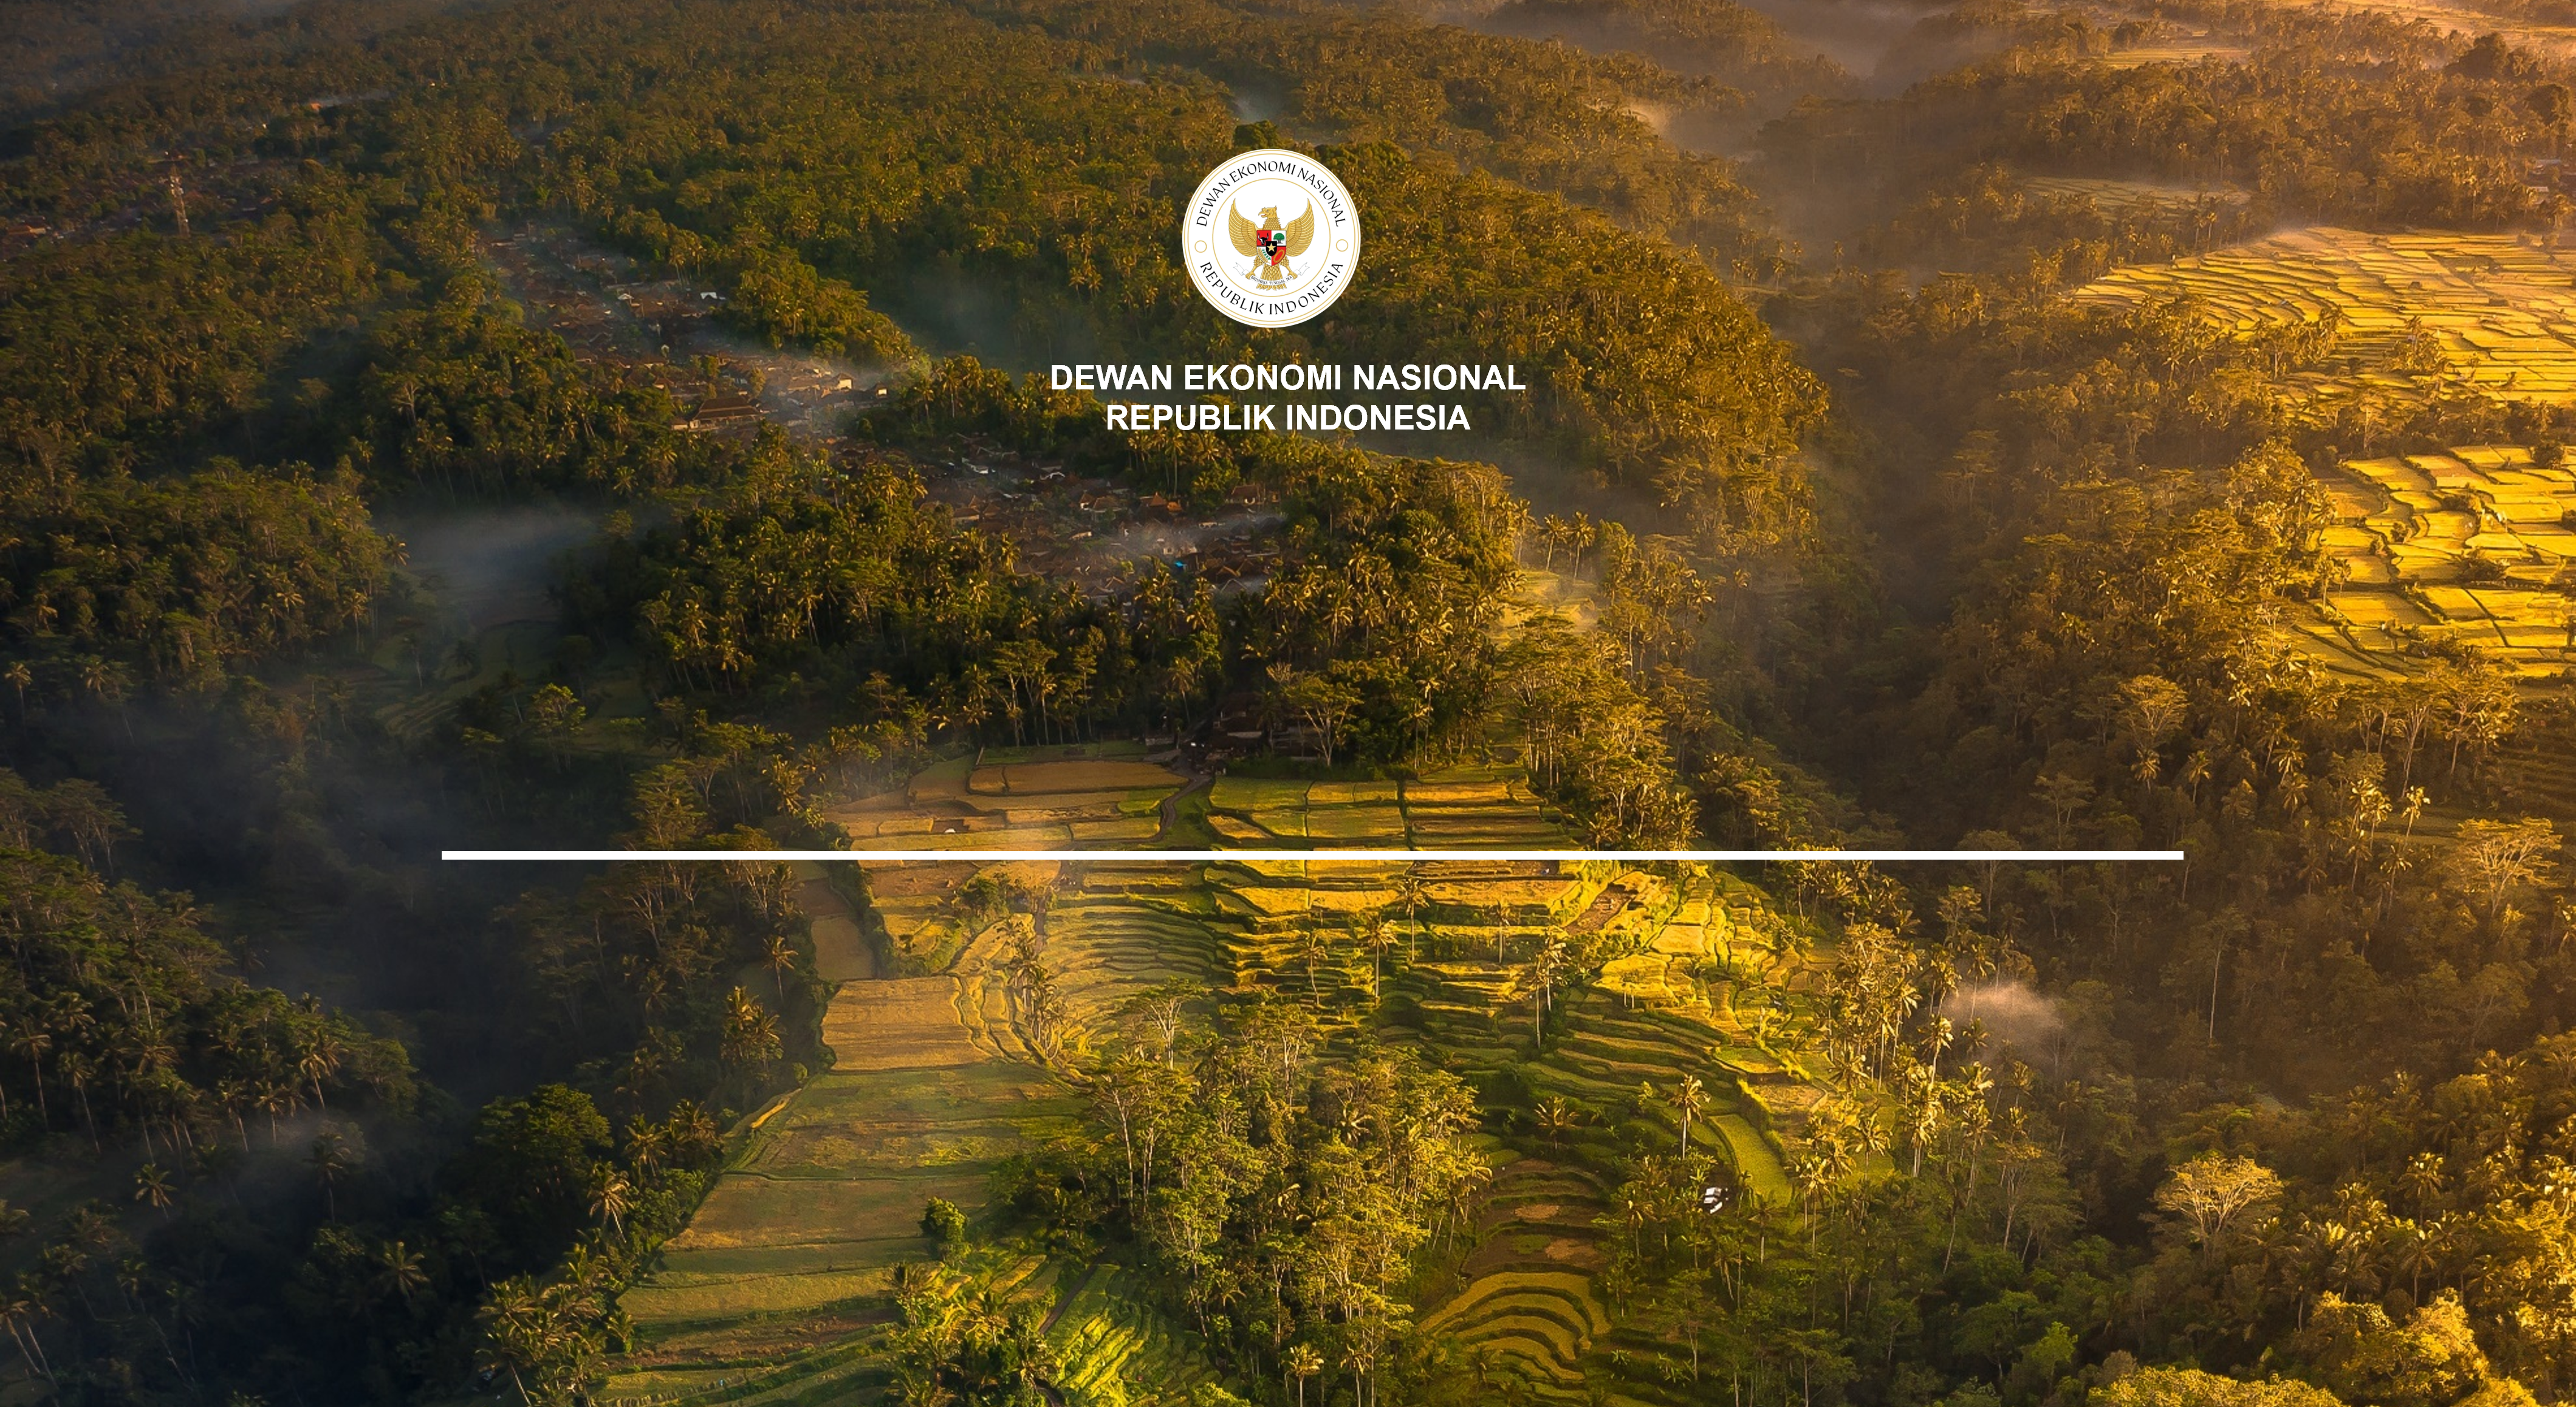
\includegraphics[width=\paperwidth, height=\paperheight]{title.png}
    };
  \end{tikzpicture}
  % Calculate title width to determine if it's long
  \setlength{\titlemaxwidth}{0.80\paperwidth}
  \settowidth{\titlewidth}{\usebeamerfont{title}\inserttitle}
  %
  \ifthenelse{\lengthtest{\titlewidth > \titlemaxwidth}}%
  {% Long title (3+ lines): 25% smaller font, higher position
    \vspace{1.8cm}
    \begin{center}
      \begin{minipage}{0.85\textwidth}
        \centering
        {\fontsize{18}{22}\selectfont\bfseries\color{white}\inserttitle\par}
        \vspace{0.3cm}
        {\usebeamerfont{author}\usebeamercolor[fg]{author}\insertauthor\par}
      \end{minipage}
    \end{center}
  }{% Short title (1 line): normal font, normal position
    \vspace{3cm}
    \begin{center}
      \begin{minipage}{0.85\textwidth}
        \centering
        {\usebeamerfont{title}\usebeamercolor[fg]{title}\inserttitle\par}
        \vspace{0.3cm}
        {\usebeamerfont{author}\usebeamercolor[fg]{author}\insertauthor\par}
      \end{minipage}
    \end{center}
  }
  \vfill
  \begin{center}
    {\usebeamerfont{date}\usebeamercolor[fg]{date}\insertdate}
  \end{center}
  \vspace{0.5cm}
}

% === Frame Title Template with Vertical Brown Line ===
\setbeamertemplate{frametitle}{
  \vspace{0.4cm}
  \begin{beamercolorbox}[wd=\paperwidth, leftskip=0.5cm]{frametitle}
    \tikz[baseline=-0.3ex]{
      \fill[denbrown] (0, -0.35) rectangle (0.15, 0.55);
    }
    \hspace{0.3cm}
    \usebeamerfont{frametitle}\insertframetitle
  \end{beamercolorbox}
}

% === Logo in Top Right ===
\addtobeamertemplate{frametitle}{}{
  \begin{tikzpicture}[remember picture, overlay]
    \node[anchor=north east, xshift=-0.4cm, yshift=-0.2cm] at (current page.north east) {
      \includegraphics[height=1cm]{logo.png}
    };
  \end{tikzpicture}
}

% === Footer with Page Number (Brown Box Bottom Right Corner) ===
\setbeamertemplate{footline}{
  \begin{tikzpicture}[remember picture, overlay]
    \node[
      anchor=south east, 
      fill=denbrown, 
      text=white,
      inner sep=4pt,
      minimum width=0.6cm,
      minimum height=0.5cm,
      font=\footnotesize
    ] at (current page.south east) {
      \insertframenumber
    };
  \end{tikzpicture}
}

% === List Item Styling ===
\setbeamertemplate{itemize item}{\textcolor{denbrown}{\textbullet}}
\setbeamertemplate{itemize subitem}{\textcolor{denbrown}{\textendash}}
\setbeamertemplate{enumerate item}{\textcolor{denbrown}{\insertenumlabel.}}

% === Block Styling ===
\setbeamercolor{block title}{bg=denbrown, fg=white}
\setbeamercolor{block body}{bg=dengray, fg=dendark}

% === Ending Slide Command ===
\providecommand{\denendslide}{
  \begin{frame}[plain]
    \begin{tikzpicture}[remember picture, overlay]
      \node[anchor=center] at (current page.center) {
        
\includegraphics[width=\paperwidth, height=\paperheight]{end.png}
      };
    \end{tikzpicture}
  \end{frame}
}

% === Support for ending-slide class via background-image attribute ===
\makeatletter
\define@key{beamerframe}{background-image}{%
  \setbeamertemplate{background}{%
    \begin{tikzpicture}[remember picture, overlay]
      \node[anchor=center] at (current page.center) {
        \includegraphics[width=\paperwidth, height=\paperheight]{#1}
      };
    \end{tikzpicture}
  }%
}
\makeatother

% === Small Slide Classes for Heavy Content ===
% \small and \footnotesize are used via Lua filter
% These environments provide additional control if needed
\newenvironment{smallslide}{\small}{}
\newenvironment{smallerslide}{\footnotesize}{}
